\documentclass[14pt, oneside]{article}     	% use "amsart" instead of "article" for AMSLaTeX format
\usepackage{geometry}                		% See geometry.pdf to learn the layout options. There are lots.

\geometry{left=25mm,right=25mm,top=30mm,bottom=30mm}
\geometry{letterpaper}                   		% ... or a4paper or a5paper or ...
%\geometry{landscape}                		% Activate for rotated page geometry
%\usepackage[parfill]{parskip}    		% Activate to begin paragraphs with an empty line rather than an indent
\usepackage[dvipdfmx]{graphicx}				% Use pdf, png, jpg, or eps§ with pdflatex; use eps in DVI mode
								% TeX will automatically convert eps --> pdf in pdflatex
\usepackage{amssymb}

\usepackage{listings}
\renewcommand{\lstlistingname}{コード}
%SetFonts
\lstset{%
  language={vhdl},
  basicstyle={\small},%
  identifierstyle={\small},%
  commentstyle={\small\itshape},%
  keywordstyle={\small\bfseries},%
  ndkeywordstyle={\small},%
  stringstyle={\small\ttfamily},
  frame={single},
  breaklines=true,
  columns=[l]{fullflexible},%
  numbers=left,%
  xrightmargin=0zw,%
  xleftmargin=3zw,%
  numberstyle={\scriptsize},%
  stepnumber=1,
  numbersep=1zw,%
  lineskip=-0.5ex%
}
%SetFonts


\title{並列分散処理  最終レポート}
\author{大城 慶知}
%\date{}							% Activate to display a given date or no date

\begin{document}
\maketitle

\section{テーマ}
Pythonにおける非同期処理を用いたI/Oの並列処理を行う。
\section{Python並列処理の基礎知識}

\subsection{スレッドの制約}
Pythonでは、GIL(Global Interpreter Lock)と呼ばれる制約がある。
GILとは、Pythonを実行した際に一つだけしかスレッドのリソースを起動できない制約である。
そのため、PythonのCPUバウンドの並列処理はプロセスを使って、I/Oバウンドの並列処理はスレッドを行う事が多い。

\begin{figure}[h]
  \centering
  \includegraphics[width=10cm]{multithred_iobound.png}
  \caption{林檎の図}
\end{figure}

\begin{figure}[h]
  \centering
  \includegraphics[width=10cm]{multithred_cpubound.png}
  \caption{林檎の図}
\end{figure}


\begin{figure}[h]
  \centering
  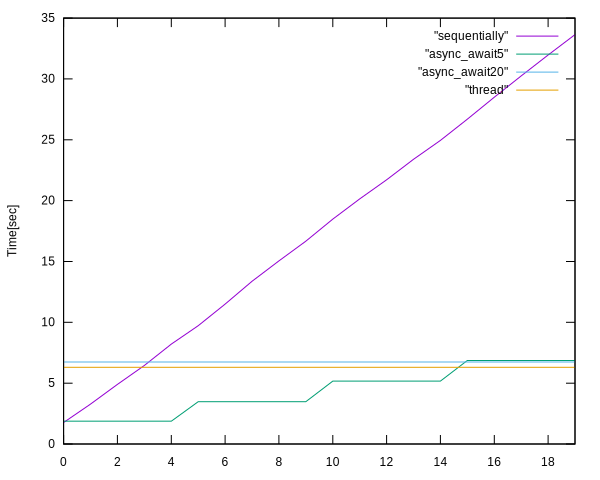
\includegraphics[width=10cm]{time.png}
  \caption{林檎の図}
\end{figure}

\subsection{プロセスを用いた}


\begin{lstlisting}[caption=シンプレクス法プログラム]

\end{lstlisting}


\section{動作確認}

\vspace{5mm}


\begin{center}
  \begin{table}[htb]
    \begin{tabular}{|l|c|} \hline
      ボタン名 & 動作 \\ \hline \hline
      SW1 & スタート・ストップ \\ \hline
      SW2 & リセット \\ \hline
      SW3 & LAPボタン \\ \hline
    \end{tabular}
  \end{table}
\end{center}


\vspace{5mm}





\section{感想・意見}

\begin{thebibliography}{9}
  \bibitem{harris} Pythonをとりまく並行/非同期の話,  https://tell-k.github.io/pyconjp2017/
  \bibitem{susan} S. M. Smith and J. M. Brady,
    ``SUSAN|A new approach to low level image processing,'' Int. J. Comput.
    Vis., vol.23, no.1, pp.45-78, May 1997.
\end{thebibliography}


\end{document}
